% introduction à la théorie des graphes

\begin{frame}{Pourquoi étudier les graphes ?}
    \begin{itemize}
        \item Les graphes sont des objets abstraits permettant de modéliser de nombreux problèmes
        \begin{itemize}
            \item de la vie courante 
            \item algorithmiques 
        \end{itemize}
        \item Il existe de nombreux algorithmes pour résoudre ces problèmes
        \item Note : il existe de nombreux problèmes difficiles à résoudre 
    \end{itemize}
\end{frame}


\begin{frame}{Les graphes sont partout !}
    Exemple : graphe des liens Facebook (10 millions de n\oe uds sur les 500 millions d'utilisateurs en 2010)
    \begin{center}
        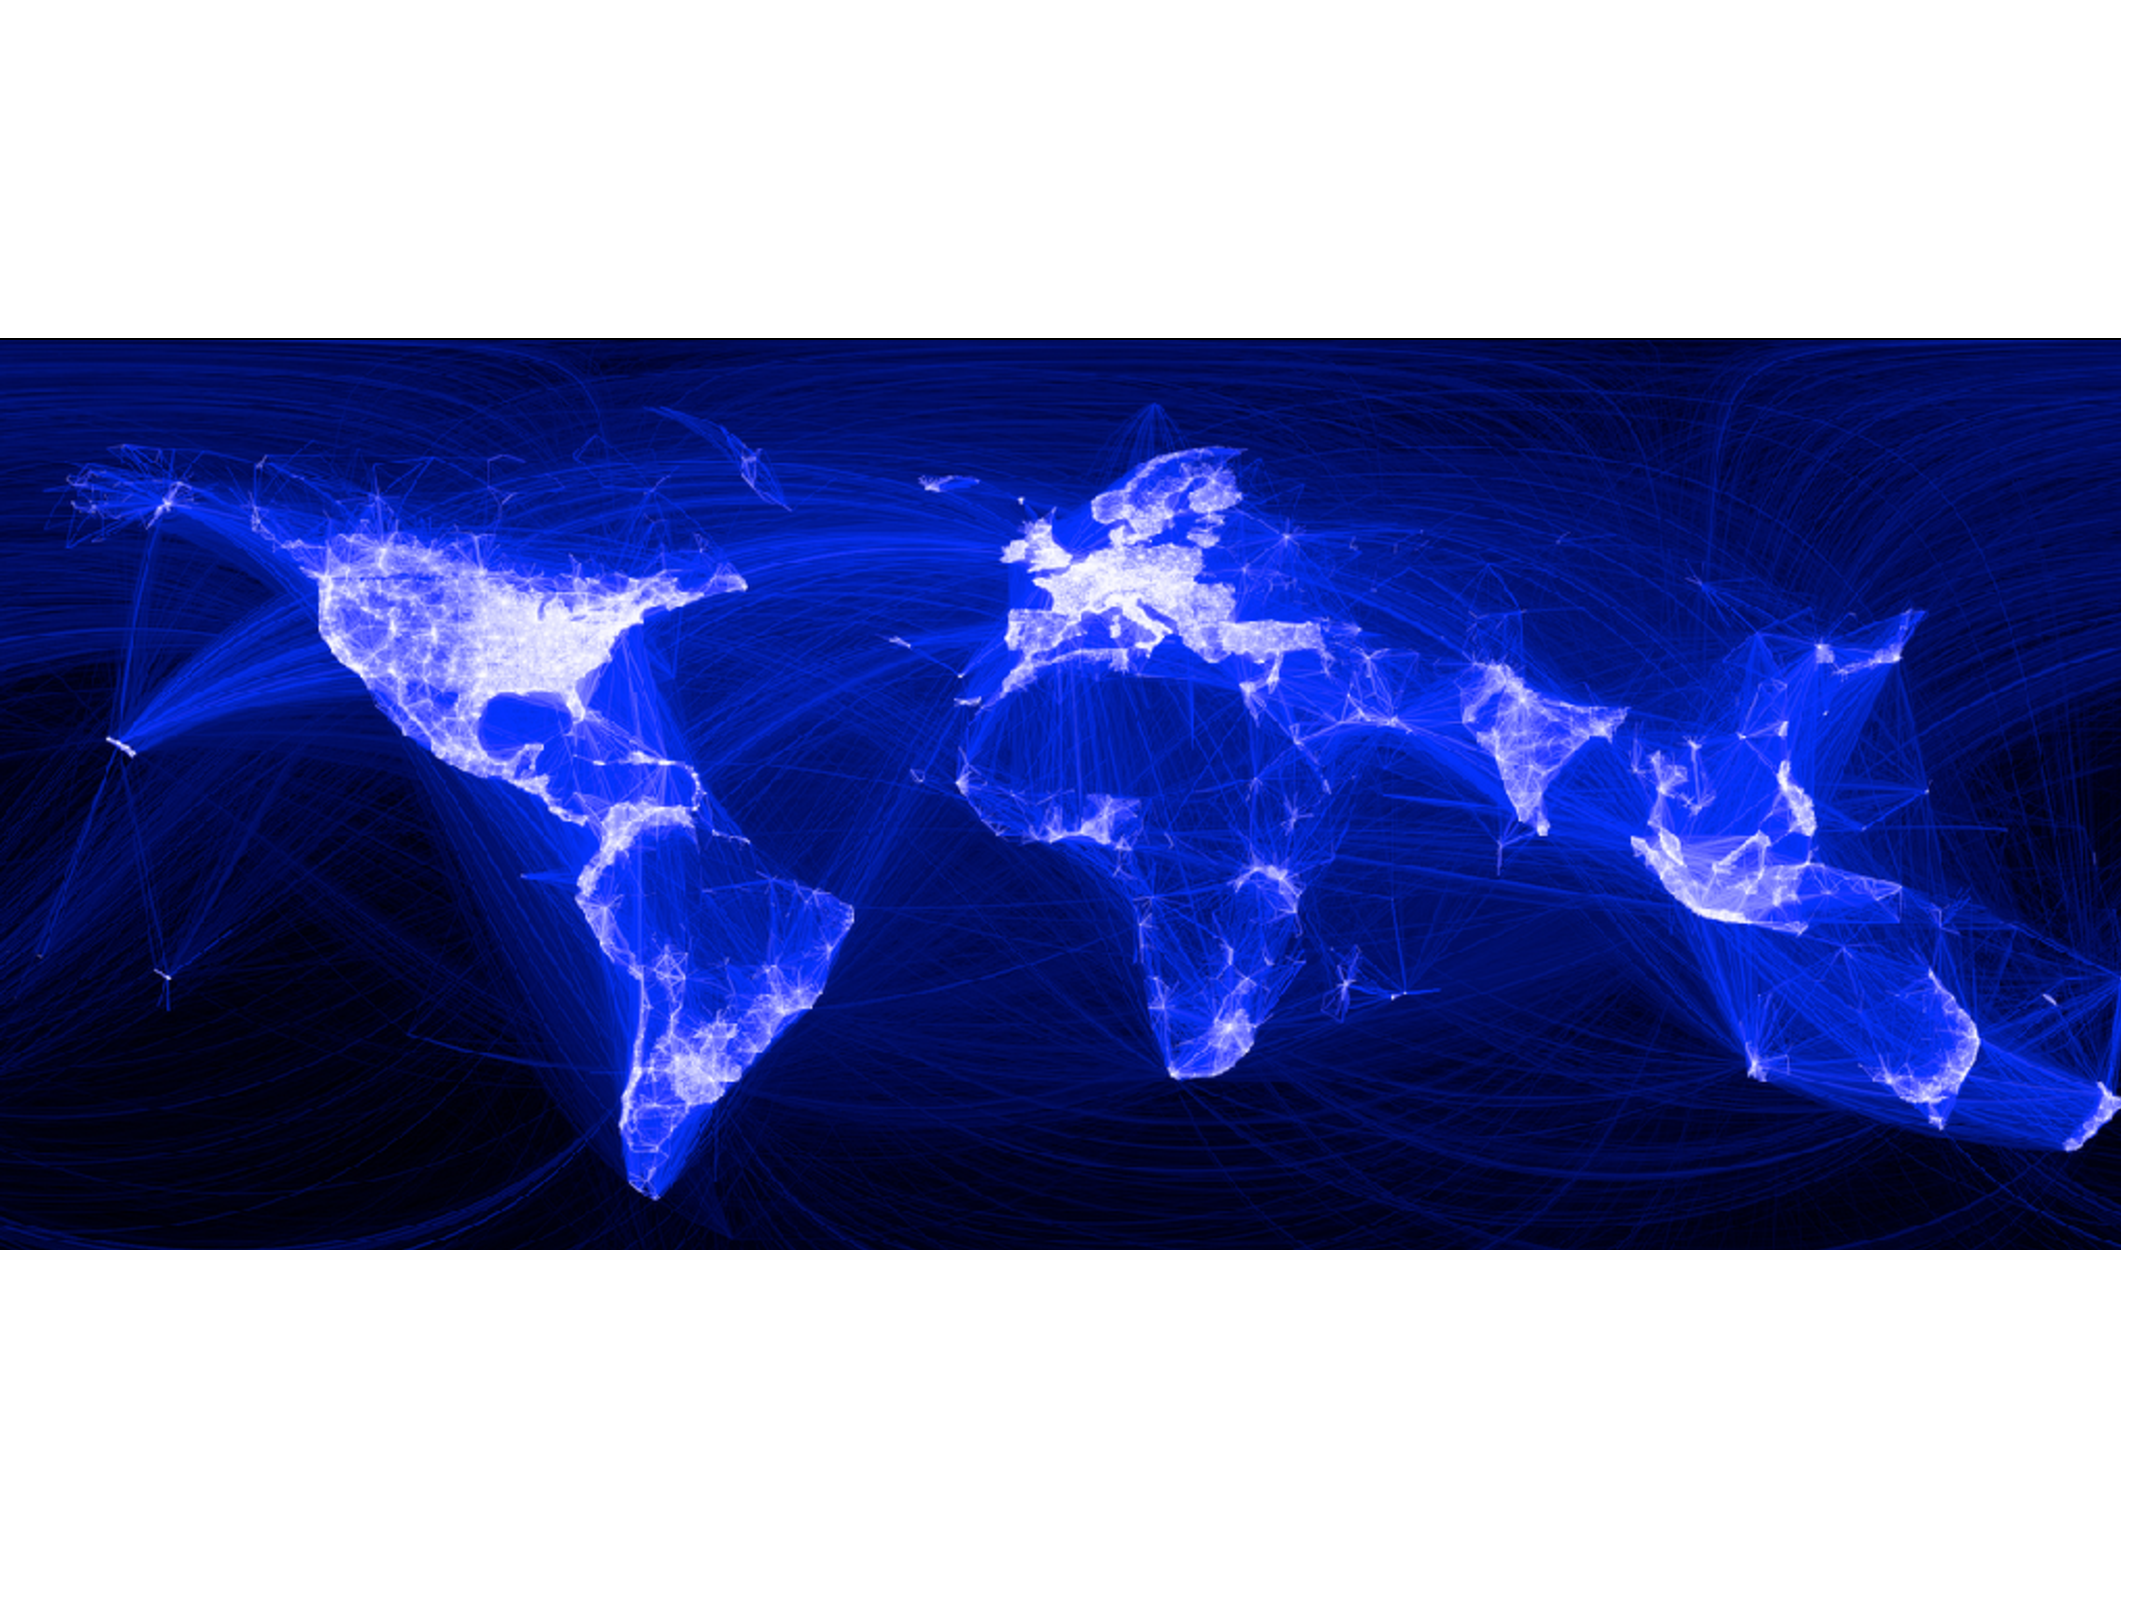
\includegraphics[width=\textwidth]{fig/facebook.pdf}
    \end{center}
\end{frame}

\begin{frame}{Réseau de transport}
    \begin{center}
        \includegraphics[width=\textwidth]{fig/tan.pdf}
    \end{center} 
\end{frame}

\begin{frame}{Quelles questions à résoudre ?}
    \begin{itemize}
        \item Atteignabilité : existe-t-il un itinéraire de l'Ecole Centrale à l'aéroport ?
        \begin{itemize}
            \item Dans un automate à état finis : un état est-il atteignable, un programme termine-t-il toujours, etc...
        \end{itemize}
        \item "Meilleur chemin" : quel est le chemin le plus court en distance(respectivement en temps, en coût...) pour aller de $A$ à $B$  ? Et en tenant compte du trafic ? Avec quelle puissance de calcul ?
        \item Isochrones : quels sont les lieux situés à moins de 15 minutes de trajet ? 
        \item Pour aller plus loin : notion de capacité et de flot 
        \begin{itemize}
            \item Combien de personnes peut-on transporter de $A$ à $B$ étant donné la capacité des trams / bus / voitures individuelles ? 
            \item Comment minimiser le coût ?
        \end{itemize}
    \end{itemize}
\end{frame}

\begin{frame}{A l'origine d'Internet : ARPAnet}
    \begin{center}
        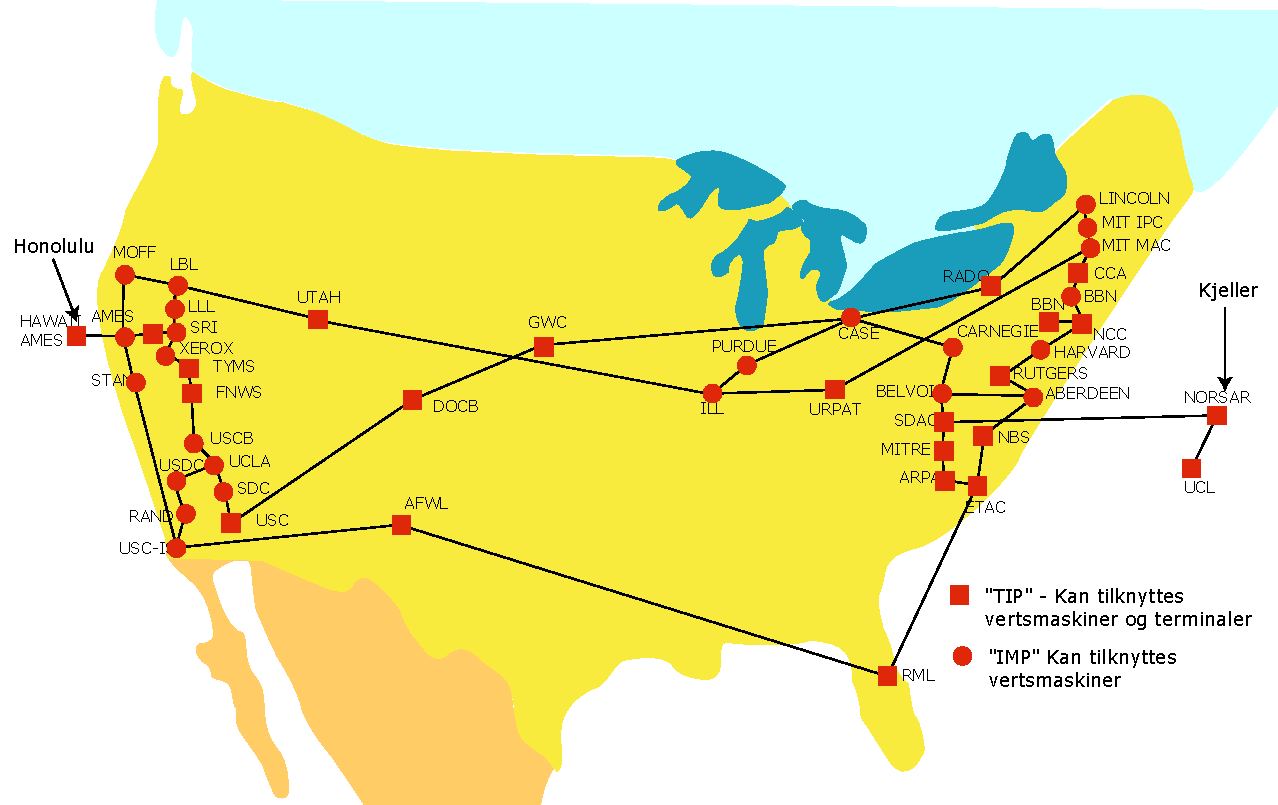
\includegraphics[width=6cm]{fig/Arpanet_1974.pdf}
    \end{center}
    \begin{itemize}
        \item Ancêtre d'Internet 
        \item Réseau décentralisé, capacité à communiquer en dépit de coupures 
        \begin{itemize}
            \item Des coupures plus critiques que d'autres ?
            \item Combien de coupures max ?
        \end{itemize}
    \end{itemize}
\end{frame}

\begin{frame}{Problème du voyageur de commerce}
    Problème : calculer un plus court circuit qui passe une et une seule fois par chaque sommet
\begin{center}
    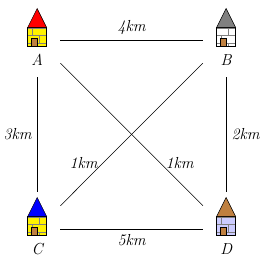
\includegraphics[width=3cm]{fig/Tsp_instance.png}
    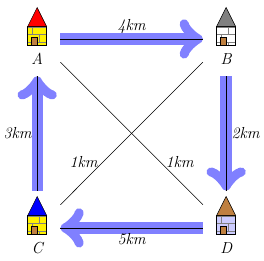
\includegraphics[width=3cm]{fig/Tsp_solution_debile.png}
    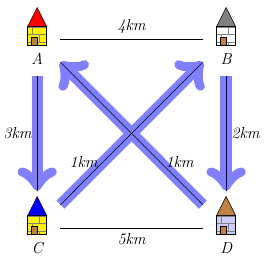
\includegraphics[width=3cm]{fig/Tsp_opt.png}
\end{center}
\begin{itemize}
    \item Problème NP-complet 
    \item Algorithme naïf en ${\cal O}(n!)$, il existe une solution en ${\cal O}(n^2 2^n)$ [Hedel et Karp, 1962]
    \item Nécessité d'avoir des solutions approchées 
\end{itemize}
\end{frame}

\begin{frame}{Makefile : graphe de dépendance}
    \begin{center}
        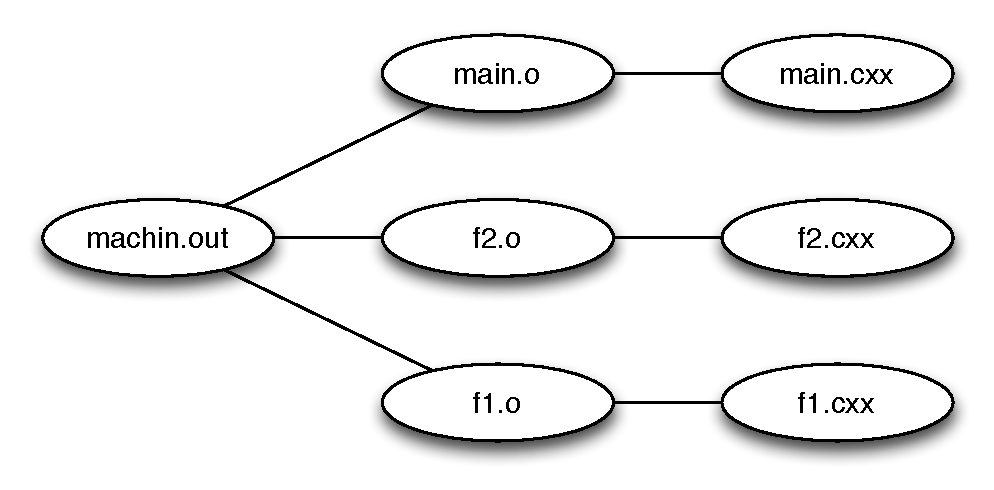
\includegraphics[width=.7\textwidth]{fig/base-dependance.pdf}
    \end{center}
\end{frame}
\begin{frame}{Makefile : graphe de dépendance}
    \begin{center}
        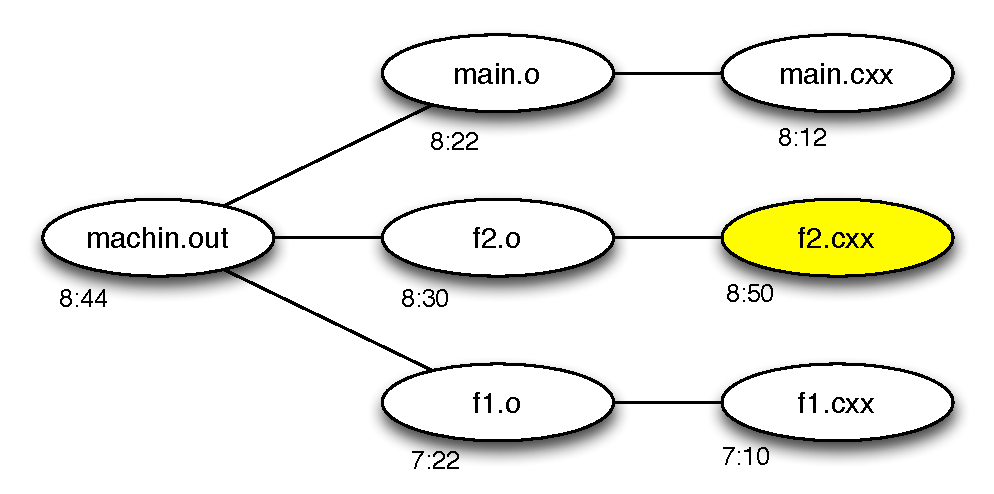
\includegraphics[width=.7\textwidth]{fig/base-dependance1.pdf}
    \end{center}
\end{frame}
\begin{frame}{Makefile : graphe de dépendance}
    \begin{center}
        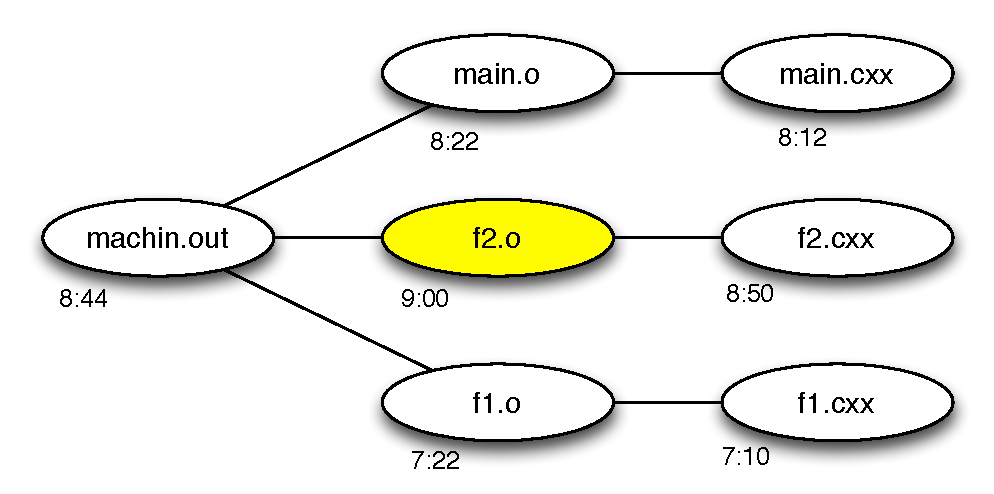
\includegraphics[width=.7\textwidth]{fig/base-dependance2.pdf}
    \end{center}
\end{frame}
\begin{frame}{Makefile : graphe de dépendance}
    \begin{center}
        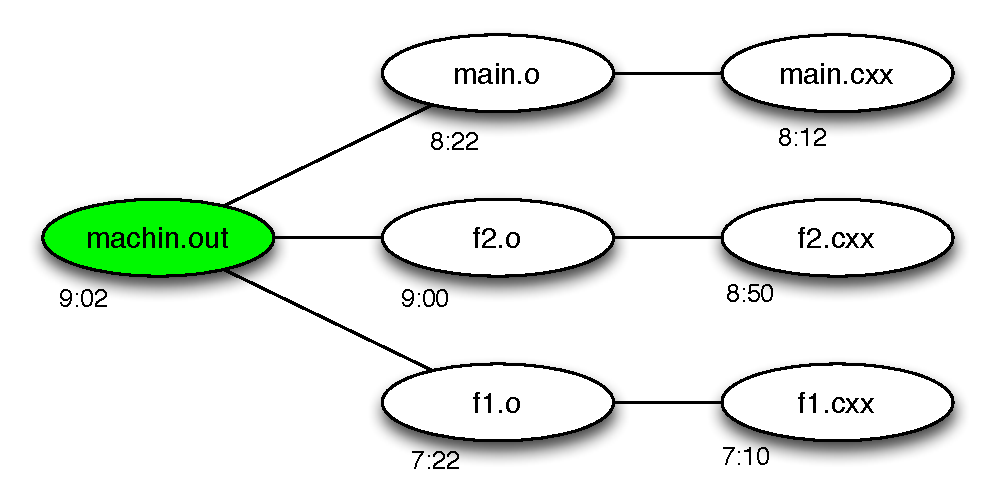
\includegraphics[width=.7\textwidth]{fig/base-dependance3.pdf}
    \end{center}
\end{frame}

\begin{frame}{"Intelligence artificielle" : jeux}
    \begin{center}
        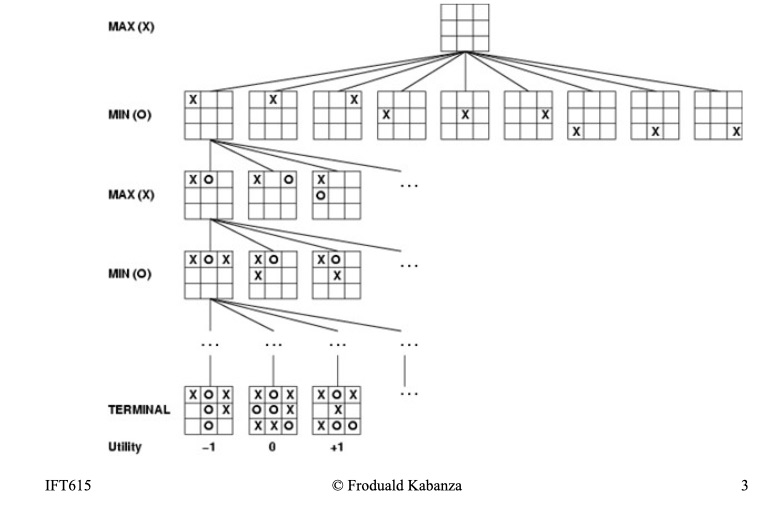
\includegraphics[width=.9\textwidth]{fig/morpion.jpg}
    \end{center} 
\end{frame}

\begin{frame}{k-coloration}
Quel est le nombre de couleurs minimum qu'il faut utiliser pour colorier les départements de façon à ce deux départements adjacents ne soient jamais de la même couleur ?
\begin{center}
    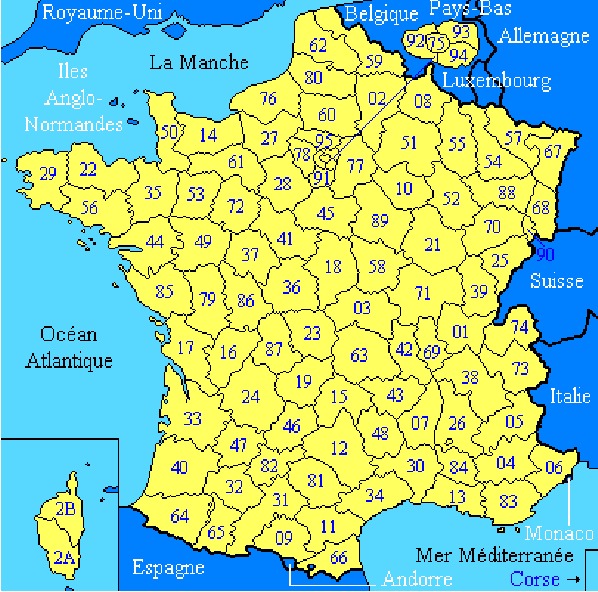
\includegraphics[width=.5\textwidth]{fig/france.pdf}
\end{center} 
\begin{itemize}
    \item Un graphe planaire (sommet = département, arc = adjacence) est 4-colorable 
    \item Application pour le parallélisme et les graphes de dépendance 
\end{itemize}
\end{frame}